%\documentclass[handout]{beamer} 
\documentclass[t,12pt,numbers,fleqn]{beamer}
%\documentclass[ignorenonframetext]{beamer}

\newif\ifquestions
%\questionstrue
\questionsfalse

\usepackage{pgfpages} 
\usepackage{hyperref}
\hypersetup{colorlinks=true,
    linkcolor=blue,
    citecolor=blue,
    filecolor=blue,
    urlcolor=blue,
    unicode=false}
\urlstyle{same}

\usepackage{booktabs}
\usepackage{hhline}
\usepackage{multirow}
\usepackage{multicol}
\usepackage{array}
\usepackage{listings}
\usepackage{bm}
\usepackage{colortbl}
\usepackage{bnf}
\newcommand{\colA}{2.1cm}
\newcommand{\colB}{6.9cm}
\newcommand{\colC}{1.1cm} %do not need this column if binding time is not listed
\newcommand{\colAwidth}{0.15\textwidth}
\newcommand{\colBwidth}{0.7\textwidth}

\newcounter{temp}
\setcounter{temp}{0}

\bibliographystyle{plain}

%\usetheme{Iimenau}

\useoutertheme{split} %so the footline can be seen, without needing pgfpages

%\pgfpagesuselayout{resize to}[letterpaper,border shrink=5mm,landscape]  %if this is uncommented, the hyperref links do not work

\mode<presentation>{}

\input{../def-beamer}

\newcommand{\topic}{05 Program Families}

%Title page information for 1D04 lectures slides

% Define year specific parameters - used in title page and footer

\newcommand{\season}{Fall} %use to switch between Winter and Fall
\newcommand{\instructor}{Dr.~Spencer Smith} %use to switch instructor
\newcommand{\instructSmall}{Dr.~Smith}
\newcommand{\yr}{2019}
\newcommand{\courseCode}{CAS 741, CES 741}
\newcommand{\courseTitle}{Development of Scientific Computing Software}

%\setbeamerfont{structure}{series=\bfseries}
%\usefonttheme[stillsansseriftext,stillsansserifmath]{serif}
\setbeamertemplate{navigation symbols}{} 
\setbeamertemplate{itemize item}[ball]

\title{
  {\normalsize \bf 
    \borange{\courseCode~(\courseTitle)\\ \season~\yr}}\\[2ex]
  {\Large \bf \topic}}

\author[Smith]{\instructor}

\institute{
  Faculty of Engineering,
  McMaster University}

\date{
\today
%January 2011\\
\bc
  \includegraphics[scale = 0.2, keepaspectratio]
  {../mcmaster-logo-full-color.jpg}
\ec
}

\renewcommand{\borange}[1] %orange is too hard to read
{
   \bred{#1}
}

\begin{document}

\input{../footline}

%%%%%%%%%%%%%%%%%%%%%%%%%%%%%%%%%%%%%%%%%%%%%%%%%%%%%%

\begin{frame}
\frametitle{Program Families}

\bi
\item Administrative details
\item Questions?
\item Finish up on SRS
\item Specification Qualities
\item Motivation
\item Proposed Family Methods
\item Family of Mesh Generators
\item Family of Linear Solvers
\item Family of Material Behaviour Models
\ei
\end{frame}

%%%%%%%%%%%%%%%%%%%%%%%%%%%%%%%%%%%%%%%%%%%%%%%%%%%%%%

\begin{frame}
\frametitle{Administrative Details}

\bi
\item Problem statement should be clear on input and output
\item Presentations
\bi
\item VGA by default, ask if need adapter
\item Can use my laptop
\ei
\item Do NOT reproduce all of the cas 741 repo in your repo, just the blank
  project template (moved to the top level)
\item Use the same names as the original
\item Delete example text from templates
\item 80 columns in tex files
\item Spell check
\item Replace ``in order to'' by ``to''
\item Use a \texttt{.gitignore} file
\item Look at \href{https://gitlab.cas.mcmaster.ca/smiths/cas741/blob/master/Repos.xlsx}{work of class mates}
\ei

\end{frame}

%%%%%%%%%%%%%%%%%%%%%%%%%%%%%%%%%%%%%%%%%%%%%%%%%%%%%%

\begin{frame}
\frametitle{Administrative Details: Deadlines}
~\newline
\begin{tabular}{l l l}
\textbf{Problem Statement} & Week 02 & Sept 15\\
\textbf{SRS Present} & Week 04 & Week of Sept 25\\
\textbf{SRS} & Week 05 & Oct 4\\
V\&V Present & Week 06 & Week of Oct 16\\
V\&V Plan & Week 07 & Oct 25\\
MG Present & Week 08 & Week of Oct 30\\
MG & Week 09 & Nov 8\\
MIS Present & Week 10 & Week of Nov 13\\
MIS & Week 11 & Nov 22\\
Impl.\ Present & Week 12 & Week of Nov 27\\
Final Documentation & Week 13 & Dec 6\\
\end {tabular}

\end{frame}

%%%%%%%%%%%%%%%%%%%%%%%%%%%%%%%%%%%%%%%%%%%%%%%%%%%%%%

\begin{frame}
\frametitle{Administrative Details: Presentation Schedule}

\bi
\item{SRS Present}
\bi
\item Tuesday: Paul, Isobel, Keshav
\item Friday: Devi, Shushen, Xiaoye
\ei
\item V\&V Present
\bi
\item Tuesday: Steven, Alexandre P., Alexander S.
\item Friday: Geneva, Jason, Yuzhi
\ei
\item MG Present
\bi
\item Tuesday: Xiaoye, Shushen, Devi, Keshav, \structure{Alex P}, Paul
\item Friday: Yuzhi, Jason, Geneva, Alex S, \structure{Isobel}, Steven
\ei
\item MIS Present
\bi
\item Tuesday: Isobel, Keshav, Paul
\item Friday: Shushen, Xiaoye, Devi
\ei
\item Impl.\ Present
\bi
\item Tuesday: Alexander S., Steven, Alexandre P.
\item Friday: Jason, Geneva, Yuzhi
\ei

\ei

\end{frame}

%%%%%%%%%%%%%%%%%%%%%%%%%%%%%%%%%%%%%%%%%%%%%%%%%%%%%%

\begin{frame}
\frametitle{Questions?}
\begin{itemize}
\item Questions about problem statements?
\item Questions about SRS?
\end{itemize}
\end{frame}

%%%%%%%%%%%%%%%%%%%%%%%%%%%%%%%%%%%%%%%%%%%%%%%%%%%%%%

\frame{\frametitle{More on the Template}
\begin{itemize}%[<+-| alert@+>]%[iacolor=gray]
\item Why a new template?
\item The new template
\begin{itemize}
\item Overview of changes from existing templates
\item Goal $\rightarrow$ Theoretical Model $\rightarrow$ Instanced Model hierarchy
\item Traceability matrix
\item System behaviour, including input constraints
\end{itemize}
\end{itemize}
}

%%%%%%%%%%%%%%%%%%%%%%%%%%%%%%%%%%%%%%%%%%%%%%%%%%%%%%

\frame{\frametitle{Why a New Template?}
From \cite{SmithAndLai2005, Lai2004}
\begin{enumerate}%[<+-| alert@+>]%[iacolor=gray]
%\item Reasons for a new template also form principles for its design
\item One user viewpoint for the physical model
\item Assumptions distinguish models
\item High potential for reuse of functional requirements
\item Characteristic hierarchical nature facilitates change
\item Continuous mathematics presents a challenge
\end{enumerate}
}

%%%%%%%%%%%%%%%%%%%%%%%%%%%%%%%%%%%%%%%%%%%%%%%%%%%%%%

\frame{\frametitle{Overview of the New Template}

\begin{itemize}

\item{Reference Material}

\item{Introduction:} 
{a) Purpose of the Document}
{b) Scope of the Software Product}
{c) Organization of the Document}

\item General System Description:
{a) System Context}
{b) User Characteristics}
{c) System Constraints}

\item \structure<2->{Specific System Description:
a) Problem Description 
b) Solution Characteristics Specification
c) Non-functional Requirements}

\item{Other System Issues}

\item \structure<2->{Traceability Matrix}

\item List of Possible Changes in the Requirements

\item{Values of Auxiliary Constants}

\item{References}

\end{itemize}
}

%%%%%%%%%%%%%%%%%%%%%%%%%%%%%%%%%%%%%%%%%%%%%%%%%%%%%%

\begin{frame}
\frametitle{Excerpts from Specific System Description}

\begin{itemize}

\item Problem Description
\begin{itemize}
\item Physical system description (\textbf{PS}) 
\item Goals (\textbf{G})
\end{itemize}
 
\item Solution Characteristics Specification
\begin{itemize}
\item Assumptions (\textbf{A})
\item Theoretical models (\textbf{T})
\item Data definitions
\item Instanced models (\textbf{M})
\item Data constraints
\item System behaviour
\end{itemize}

\item Non-functional Requirements
\begin{itemize}
\item Accuracy of input data
\item Sensitivity of the model
\item Tolerance of the solution
\item Solution validation strategies (now moved to a separate document)
\end{itemize}

\end{itemize}

\end{frame}

%%%%%%%%%%%%%%%%%%%%%%%%%%%%%%%%%%%%%%%%%%%%%%%%%%%%%%

\begin{frame}
\frametitle{Refinement from Abstract to Concrete}

\begin{overlayarea}{\textwidth}{5.3cm}
\begin{figure}[H]
\includegraphics<1>[scale=0.41]{../Figures/RefinementHierarchy.pdf}
\includegraphics<2>[scale=0.41]{../Figures/RefinementG1.pdf}
\includegraphics<3>[scale=0.41]{../Figures/RefinementT11.pdf}
\includegraphics<4>[scale=0.41]{../Figures/RefinementM111.pdf}
\includegraphics<5>[scale=0.41]{../Figures/RefinementT12.pdf}
\end{figure}
\end{overlayarea}

\begin{overlayarea}{\textwidth}{1cm}

\only<2>{\textbf{G1}: Solve for unknown forces}

\only<3>{
\begin{center} 
$%\begin{displaymath}
\mathbf{(T1_1)}~\left\{ 
\begin{array}{lll}
\textrm{$\sum{F_{xi}} = 0$}\\  
\textrm{$\sum{F_{yi}} = 0$}\\
\textrm{$\sum{M_i} = 0$}\\
\end{array} \right. $%\end{displaymath}
\end{center}
}

\only<4>{
\begin{center} $%\begin{displaymath}
\textbf{(M1)}~\left\{ 
\begin{array}{lll}
\textrm{$F_{ax} - F_1\cdot \cos\theta_3 - F_2\cdot \cos\theta_4 - F_{bx} = 0$} \\ 
\textrm{$F_{ay} - F_1\cdot \sin\theta_3 - F_2\cdot \sin\theta_4 + F_{by} = 0$}\\
\textrm{$- F_1\cdot x_1\sin\theta_3 - F_2\cdot x_2\sin\theta_4 + F_{by}\cdot L = 0$}\\
\end{array} \right. 
$%\end{displaymath}
\end{center}
}

\only<5>{
The virtual work done by all the external forces and couples acting on the system is zero for each independent virtual
displacement of the system, or mathematically $\delta U = 0$
}
\end{overlayarea}

\end{frame}

%%%%%%%%%%%%%%%%%%%%%%%%%%%%%%%%%%%%%%%%%%%%%%%%%%%%%%

\begin{frame}
\frametitle{Other goals and models}
\begin{itemize}
\item \textbf{G2}: Solve for the functions of shear force and bending moment along the beam
\item \textbf{G3}: Solve for the function of deflection along the beam
\item $\mathbf{T3_1}$: $\frac{d^2 y}{d x^2} = \frac{M}{EI}$, $y(0) = y(L) = 0$
\item $\mathbf{T3_2}$: $y$ determined by moment area method
\item $\mathbf{T3_3}$: $y$ determined using Castigliano's theorem
\item $\mathbf{M3_{11}}$: $y = \frac{12 \int_0^L (\int_0^L M dx) dx}{Eeh^3}$, $y(0) = y(L) = 0$
\end{itemize}
\end{frame}

%%%%%%%%%%%%%%%%%%%%%%%%%%%%%%%%%%%%%%%%%%%%%%%%%%%%%%

\begin{frame}
\frametitle{Kreyman and Parnas Five Variable Model}
\begin{itemize}
\item See \cite{KreymanAndParnas2002}
\item An alternative approach
\item Unfortunately the numerical algorithm is not hidden in the requirements specification
\item The analogy with real-time systems leads to some confusion
\end{itemize}
\end{frame}

%%%%%%%%%%%%%%%%%%%%%%%%%%%%%%%%%%%%%%%%%%%%%%%%%%%%%%

\begin{frame}
\frametitle{Examples}
\begin{itemize}
\item \href{https://github.com/smiths/swhs}{Solar Water Heating System}
\item \href{https://github.com/JacquesCarette/literate-scientific-software/tree/master/CaseStudies/glass/Documentation/SRS}{GlassBR}
\end{itemize}
\end{frame}

%%%%%%%%%%%%%%%%%%%%%%%%%%%%%%%%%%%%%%%%%%%%%%%%%%%%%%

\begin{frame}
\frametitle{Summary of Template}
\begin{itemize}
\item Quality is a concern for scientific computing software
\item Software engineering methodologies can help
\item Motivated, justified and illustrated a method of writing requirements specification for engineering computation
to improve reliability
\item Also improve quality with respect to usability, verifiability, maintainability, reusability and portability
\item Tabular expressions to reduce ambiguity, encourage systematic approach
\item Conclusions can be generalized because other computation problems follow the same pattern of \emph{Input} then
\emph{Calculate} then \emph{Output}
\item Benefits of approach should increase as the number of details and the number of people involved increase
\end{itemize}
\end{frame}

%%%%%%%%%%%%%%%%%%%%%%%%%%%%%%%%%%%%%%%%%%%%%%%%%%%%%%

\begin{frame}
\frametitle{Summary of Template (Continued)}
\begin{itemize}
\item A new template for scientific computing has been developed
\item Characteristics of scientific software guided the design
\item Designed for reuse
\item Functional requirements split into ``Problem Description'' and ``Solution Characteristics Specification''
\item Traceability matrix
\item Addresses nonfunctional requirements (but room for improvement)
\end{itemize}

\end{frame}

%%%%%%%%%%%%%%%%%%%%%%%%%%%%%%%%%%%%%%%%%%%%%%%%%%%%%%

\begin{frame}
\frametitle{Specification Qualities}

\begin{itemize}

\item \structure{What are the important qualities for a specification?}

\end{itemize}

\end{frame}

%%%%%%%%%%%%%%%%%%%%%%%%%%%%%%%%%%%%%%%%%%%%%%%%%%%%%%

\begin{frame}
\frametitle{Specification Qualities}

\begin{itemize}
\item The qualities we previously discussed (usability, maintainability,
  reusability, verifiability etc.)
\item Clear, unambiguous,  understandable
\item Consistent
\item Complete
\begin{itemize}
\item Internal completeness
\item External completeness
\end{itemize}
\item Incremental
\item Validatable
\item Abstract
\item Traceable
\end{itemize}

Summarized in \cite[p.\ 406]{SmithAndKoothoor2016}

\end{frame}

%%%%%%%%%%%%%%%%%%%%%%%%%%%%%%%%%%%%%%%%%%%%%%%%%%%%%%

\begin{frame}
\frametitle{Clear, Unambiguous, Understandable}

\begin{itemize}

\item Specification fragment for a word-processor
\begin{itemize}
\item \structure{Selecting is the process of designating 
areas of the document that you want to 
work on. Most editing and formatting 
actions require two steps: first you 
select what you want to work on, 
such as text or graphics; then you 
initiate the appropriate action.}
\end{itemize}
\item What are the potential problems with this specification?
\begin{itemize}
\item<2-> {\alert{Can an area be scattered?}}
\item<2->{\alert{Can both text and graphics be selected?}}
\end{itemize}
\end{itemize}

\end{frame}

%%%%%%%%%%%%%%%%%%%%%%%%%%%%%%%%%%%%%%%%%%%%%%%%%%%%%%

\begin{frame}
\frametitle{Clear, Unambiguous, Understandable}

\begin{itemize}

\item Specification fragment from a real safety-critical system
\begin{itemize}
\item \structure{The message must be triplicated. The three
copies must be forwarded through three 
different physical channels. The receiver 
accepts the message on the basis of a 
two-out-of-three voting policy.}
\end{itemize}
\item What is a potential problems with this specification?
\begin{itemize}
\item<2-> {\alert{Can a message be accepted as soon as we receive 2 out of 3 identical copies, or do we need to wait
for receipt of the 3rd}}
\end{itemize}
\end{itemize}

\end{frame}

%%%%%%%%%%%%%%%%%%%%%%%%%%%%%%%%%%%%%%%%%%%%%%%%%%%%%%

\begin{frame}
\frametitle{Unambiguous, Validatable}

\begin{itemize}

\item Specification fragment for an end-user program
\begin{itemize}
\item \structure{The program shall be user friendly.}
\end{itemize}
\item What is a potential problems with this specification?
\begin{itemize}
\item<2-> {\alert{What does it mean to be user friendly?}}
\item<2-> {\alert{Who is a typical user?}}
\item<2-> {\alert{How would you measure success or failure in meeting this requirement?}}
\end{itemize}

\end{itemize}

\end{frame}

%%%%%%%%%%%%%%%%%%%%%%%%%%%%%%%%%%%%%%%%%%%%%%%%%%%%%%

\begin{frame}
\frametitle{Unambiguous, Validatable}

\begin{itemize}

\item Specification fragment for a linear solver
\begin{itemize}
\item \structure{Given $A$ and $b$, solve the  linear system $A x = b$ for $x$, such that the error in any entry of
$x$ is less than 5 \%.}
\end{itemize}
\item What is a potential problems with this specification?
\begin{itemize}
\item<2-> {\alert{Is $A$ constrained to be square?}}
\item<2-> {\alert{Can $A$ be singular?}}
\item<2-> {\alert{Even if the problem is made completely unambiguous, the requirement cannot be validated.}}
\end{itemize}

\end{itemize}

\end{frame}

%%%%%%%%%%%%%%%%%%%%%%%%%%%%%%%%%%%%%%%%%%%%%%%%%%%%%%

\begin{frame}
\frametitle{Consistent}

\begin{itemize}

\item Specification fragment for a word-processor
\begin{itemize}
\item \structure{The whole text should be kept in lines 
of equal length. The length is specified 
by the user. Unless the user gives an 
explicit hyphenation command, 
a carriage return should occur only 
at the end of a word.}
\end{itemize}
\item What is a potential problems with this specification?
\begin{itemize}
\item<2-> {\alert{What if the length of a word exceeds the length of the line?}}
\end{itemize}

\end{itemize}

\end{frame}

%%%%%%%%%%%%%%%%%%%%%%%%%%%%%%%%%%%%%%%%%%%%%%%%%%%%%%

\begin{frame}
\frametitle{Same Symbol/Term Different Meaning}

\begin{itemize}

\item \structure{Can you think of some symbols/terms that have different
    meanings depending on the context?}

\end{itemize}

\end{frame}

%%%%%%%%%%%%%%%%%%%%%%%%%%%%%%%%%%%%%%%%%%%%%%%%%%%%%%

\begin{frame}
\frametitle{Consistent}

\begin{itemize}

\item Language and terminology must be consistent within the specification
\item Potential problem with homonyms, for instance consider the symbol $\sigma$
\begin{itemize}
\item Represents standard deviation
\item Represents stress
\item Represents the Stefan-Boltzmann constant (for radiative heat transfer)
\end{itemize}
\item Changing the symbol may be necessary for consistency, but it could adversely effect understandability
\item Potential problem with synonyms
\begin{itemize}
\item Externally funded graduate students, versus eligible graduate students, versus non-VISA students
%ask who would think about graduate school?
\item Material behaviour model versus constitutive equation
\end{itemize}
\end{itemize}

\end{frame}

%%%%%%%%%%%%%%%%%%%%%%%%%%%%%%%%%%%%%%%%%%%%%%%%%%%%%%

\begin{frame}
\frametitle{Complete}

\begin{itemize}

\item Internal completeness
\begin{itemize}
\item The specification must define any new concept or terminology that it uses
\begin{itemize}
\item A glossary is helpful for this purpose
\end{itemize}
\end{itemize}
\item External completeness
\begin{itemize}
\item The specification must document all the needed requirements
\begin{itemize}
\item Difficulty: when should one stop?
\end{itemize}
\end{itemize}

\end{itemize}

\end{frame}

%%%%%%%%%%%%%%%%%%%%%%%%%%%%%%%%%%%%%%%%%%%%%%%%%%%%%%

\begin{frame}
\frametitle{Incremental}

\begin{itemize}

\item Referring to the specification process
\begin{itemize}
\item Start from a sketchy document and progressively add details
\item A document template can help with this
\end{itemize}
\item Referring to the specification document
\begin{itemize}
\item Document is structured and can be understood in increments
\item Again a document template can help with this
\end{itemize}

\end{itemize}

\end{frame}

%%%%%%%%%%%%%%%%%%%%%%%%%%%%%%%%%%%%%%%%%%%%%%%%%%%%%%

\begin{frame}
\frametitle{Traceable}

\begin{itemize}

\item Explicit links
\bi
\item Within document
\item Between documents
\ei
\item Use labels, cross-references, traceability matricies
\item Common sense suggests traceability improves maintainability
\item Shows consequence of change
\item Minimizes cost of recertification
\item Additional advantages
\bi
\item Program comprehension
\item Impact analysis
\item Reuse
\ei
\end{itemize}

\end{frame}

%%%%%%%%%%%%%%%%%%%%%%%%%%%%%%%%%%%%%%%%%%%%%%%%%%%%%%

\begin{frame}
\frametitle{Accuracy Versus Precision}

\begin{center}
 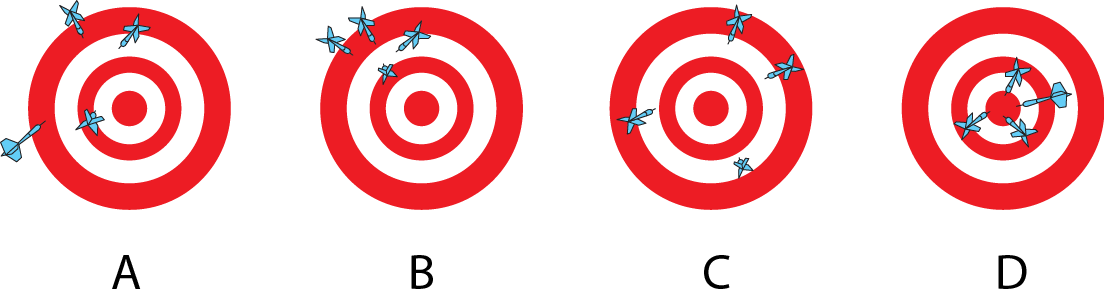
\includegraphics[width=1.0\textwidth]{../Figures/AccuracyPrecision_FromUniversityOfHawaiiAtManoa.png}
\end{center}

\structure{What is the distinction between accuracy and precision?}

\end{frame}

%%%%%%%%%%%%%%%%%%%%%%%%%%%%%%%%%%%%%%%%%%%%%%%%%%%%%%

\begin{frame}
\frametitle{Program Families}

\begin{itemize}

\item Can think of general purpose (or multi-purpose) SC software as a program
  family
\item Some examples of physical models are also appropriate for consideration as
  a family
\item A program family is a set of programs where it makes more sense to develop
  them together as opposed to separately
\item Analogous to families in other domains
\begin{itemize}
\item Automobiles
\item Computers
\item ...
\end{itemize}
\item Need to identify the commonalities
\item Need to identify the variabilities
\item Discussed in general in \cite{ClementsAndNorthrop2001,PohlEtAl2005}
\end{itemize}

\end{frame}

%%%%%%%%%%%%%%%%%%%%%%%%%%%%%%%%%%%%%%%%%%%%%%%%%%%%%%

\begin{frame}
\frametitle{Background}

\begin{itemize}

\item Program family idea since the 1970s (Dijkstra, Parnas, Weiss, Pohl, ...) - variabilities are often from a finite
set of simple options \cite{Parnas1976, Parnas1979, Dijkstra1972}
\item Families of algorithms and code generation in SC (Carette, ATLAS, Blitz++, ...) - not much emphasis on
requirements \cite{Carette2006, WhaleyEtAl2001, Veldhuizen1998, Blitz2010}
%\item Problem Solving Environments (PSEs)
\item Work on requirements for SC
\begin{itemize}
\item Template for a single physical model \cite{SmithEtAl2007, SmithAndLai2005}
\item Template for a family of multi-purpose tool \cite{Smith2006,
    SmithAndChen2004, SmithAndChen2004b}
\item Template for a family of physical models
  \cite{SmithMcCutchanAndCarette2017, SmithEtAl2008, McCutchan2007}
\end{itemize}
\end{itemize}

\end{frame}

 %%%%%%%%%%%%%%%%%%%%%%%%%%%%%%%%%%%%%%%%%%%%%%%%%%%%%%

\begin{frame}

\frametitle{Motivation}
%:Improve Quality of Product and Process
\begin{itemize}

\item Requirements documentation
\begin{itemize}
\item Allows judgement of quality %need to know what require, 
\item Improves communication
\begin{itemize}
\item Between domain experts% and domain experts %missing models etc.
\item Between domain experts and programmers %experts on num algos
\item Explicit assumptions
\item Range of applicability
%\item Tradeoffs between nonfunctional requirements %ends arguments about best, 
% need to know what is most imp, might not need same accuracy for every aspect of the problem
\end{itemize}
%\item Provides a foundation for incremental delivery
\end{itemize}

\item A family approach, potentially including a DSL to allow generation of specialized programs
\begin{itemize}
\item Improves efficiency of product and process
\item Facilitates reuse of requirements and design, which improves reliability
\item Improves usability and learnability%DSL
%\item Improves learnability for non-experts %DSL
\item Clarifies the state of the art
\end{itemize}

\end{itemize}

\end{frame}

%%%%%%%%%%%%%%%%%%%%%%%%%%%%%%%%%%%%%%%%%%%%%%%%%%%%%%

\begin{frame}

\frametitle{Advantages of Program Families to SC?}

\begin{itemize}
\item Usual benefits
\begin{itemize}
\item Reduced development time
\item Improved quality
\item Reduced maintenance effort
\item Increased ability to cope with complexity
\end{itemize}
\item Reusability
\begin{itemize}
\item Underused potential for reuse in SC
\item Reuse commonalities
\item Systematically handle variabilities
\end{itemize}
\item Usability
\begin{itemize}
\item Documentation often lacking in SC
\item Documentation part of program family methodology
\item Create family members that are only as general purpose as necessary
\end{itemize}
\item Improved performance
\end{itemize}

\end{frame}

%%%%%%%%%%%%%%%%%%%%%%%%%%%%%%%%%%%%%%%%%%%%%%%%%%%%%%

\begin{frame}

\frametitle{Is SC Suited to a Program Family Approach?}

Based on criteria from Weiss \cite{ArdisAndWeiss1997, Weiss1997, Weiss1998,
  CukaAndWeiss1997,WeissAndLai1999}
\begin{itemize}
\item The redevelopment hypothesis
\begin{itemize}
\item A significant portion of requirements, design and code should be common between family members
\item Common model of software development in SC is to rework an existing program
\item Progress is made by removing assumptions
\end{itemize}

\item The oracle hypothesis
\begin{itemize}
\item Likely changes should be predictable
\item Literature on SC, example systems, mathematics
\end{itemize}

\item The organizational hypothesis
\begin{itemize}
\item Design so that predicted changes can be made independently
\item Tight coupling between data structures and algorithms
\item Need a suitable abstraction
\end{itemize}

\end{itemize}

\end{frame}

%%%%%%%%%%%%%%%%%%%%%%%%%%%%%%%%%%%%%%%%%%%%%%%%%%%%%%

\begin{frame}

\frametitle{Challenges}

\begin{enumerate}
\setcounter{enumi}{\value{temp}}
\item Validatable
\begin{itemize}
\item Requirements can be complete, consistent, traceable and unambiguous, but still not validatable
\item Input and outputs are continuously valued variables
%\item Examples continuously valued variables: time, velocity, temperature, displacement, concentration, stress, etc.
%\item Infinite number of inputs and outputs
\item Correct solution is unknown a priori %difficult to have a test oracle
\item Given $dy/dt = f(t, y)$ and $y(t_0) = y_0$, find $y(t_n)$ 
%, where $y(t)$ is a function ($y:\mathbb{R} \rightarrow 
%\mathbb{R}$), $f(t,y)$ is a function ($f:\mathbb{R}\times \mathbb{R} \rightarrow \mathbb{R}$), $t$ is an independent
%variable (often time), $t_0$ is an initial value for $t$ and $t_n$ is the final value for $t$
%\item For arbitrary $f(t, y)$ the true solution is unknown, correct value is often not known a priori
%\item Same problem with $Ax = b$
%\item $\int e^{x^2} dx$
%\item Passing one test does not imply passing a nearby test
\end{itemize}
\item Abstract
\begin{itemize}
% \item Not difficult to be abstract
\item If too abstract, then difficult to meet NFRs for accuracy and speed
\item Assumptions can help restrict scope, but possibly as much work as solving the original problem
\begin{itemize}
\item $A x = b$
\item $x^T A x > 0, \forall x$
\end{itemize}
%say output should be solution, or say cannot compute, possibly with a reason
\item Algorithm selection should occur at the design stage

\end{itemize}

\setcounter{temp}{\value{enumi}}
\end{enumerate}

\end{frame}

%%%%%%%%%%%%%%%%%%%%%%%%%%%%%%%%%%%%%%%%%%%%%%%%%%%%%%

\begin{frame}

\frametitle{Challenges (Continued)}

\begin{enumerate}
\setcounter{enumi}{\value{temp}}
\item Nonfunctional requirements
\begin{itemize}
\item Proving accuracy requirements with a priori error analysis is a difficult mathematical exercise that generally
leads to weak error bounds
% mention Wilkinson
\item Context sensitive tradeoffs between NFRs can be difficult to specify
\item Absolute quantitative requirements are often unrealistic
% make the point about relative requirements elsewhere
\end{itemize}
\item Capture and Reuse Existing Knowledge
\begin{itemize}
\item Cannot ignore the enormous wealth of information that currently exists %not a green field development
\item A good design will often involve integrating existing software libraries
\item Reuse software and the requirements documentation
% scientific software is stable
\end{itemize}

\setcounter{temp}{\value{enumi}}
\end{enumerate}

\end{frame}

%%%%%%%%%%%%%%%%%%%%%%%%%%%%%%%%%%%%%%%%%%%%%%%%%%%%%%

\begin{frame}[allowframebreaks]
\frametitle{References}

\bibliography{../../ReferenceMaterial/References}

\end{frame}

%%%%%%%%%%%%%%%%%%%%%%%%%%%%%%%%%%%%%%%%%%%%%%%%%%%%%%

\end{document}